\let\negmedspace\undefined
\let\negthickspace\undefined

\documentclass[journal]{IEEEtran}
\usepackage[a5paper, margin=10mm, onecolumn]{geometry}
\usepackage{tfrupee}

\setlength{\headheight}{1cm}
\setlength{\headsep}{0mm}

\usepackage{gvv-book}
\usepackage{gvv}
\usepackage{cite}
\usepackage{amsmath,amssymb,amsfonts,amsthm}
\usepackage{algorithmic}
\usepackage{graphicx}
\usepackage{textcomp}
\usepackage{xcolor}
\usepackage{txfonts}
\usepackage{listings}
\usepackage{enumitem}
\usepackage{mathtools}
\usepackage{gensymb}
\usepackage{comment}
\usepackage[breaklinks=true]{hyperref}
\usepackage{tkz-euclide} 
\usepackage{listings}
\def\inputGnumericTable{}                                 
\usepackage[latin1]{inputenc}                                
\usepackage{color}                                            
\usepackage{array}                                            
\usepackage{longtable}                                       
\usepackage{calc}                                             
\usepackage{multirow}                                         
\usepackage{hhline}                                           
\usepackage{ifthen}                                           
\usepackage{lscape}
\begin{document}

\bibliographystyle{IEEEtran}
\vspace{3cm}

\title{9.4.22}
\author{EE25BTECH11010 - Arsh Dhoke}
{\let\newpage\relax\maketitle}

\renewcommand{\thefigure}{\theenumi}
\renewcommand{\thetable}{\theenumi}
\setlength{\intextsep}{10pt}
\numberwithin{equation}{enumi}
\numberwithin{figure}{enumi}
\renewcommand{\thetable}{\theenumi}

\parindent 0px
\textbf{Question}:\\
Find the value of $k$ such that the quadratic equation
kx(x-2) + 6 = 0 has equal roots. Verify your solution using graph.

\solution \\


\begin{align}
kx^2 - 2kx + 6 = 0
\end{align}

This can be represented as a conic:
\begin{align}
\vec{x}^{T}\vec{V}\vec{x} + 2\vec{u}^{T}\vec{x} + f = 0
\end{align}
where
\begin{align}
\vec{V} = \myvec{k & 0 \\ 0 & 0}, \quad
\vec{u} = \myvec{-k \\ 0}, \quad
f = 6
\end{align}
\begin{align}
\vec{x} = \vec{h} + k_i\vec{m} \\
\vec{m}=\myvec{1 \\ 0}
\end{align}

The value of $k_i$ can be found out by solving the line and conic equation

\begin{align}
(\vec{h} + k_i \vec{m})^{T} \vec{V} (\vec{h} + k_i \vec{m}) + 2\vec{u}^{T} (\vec{h} + k_i \vec{m}) + f &= 0 \\
\implies k_i^{2} \vec{m}^{T}\vec{V}\vec{m} + 2k_i \vec{m}^{T} (\vec{V}\vec{h} + \vec{u}) + \vec{h}^{T}\vec{V}\vec{h} + 2\vec{u}^{T}\vec{h} + f &= 0 \\
\text{or, } k_i^{2} \vec{m}^{T}\vec{V}\vec{m} + 2k_i \vec{m}^{T} (\vec{V}\vec{h} + \vec{u}) + g(\vec{h}) &= 0
\end{align}

Solving the above quadratic gives 
\begin{align}
k_i = \frac{1}{\vec{m}^{T}\vec{V}\vec{m}}
\brak{
    -\vec{m}^{T} (\vec{V}\vec{h} + \vec{u})
    \;\pm\;
    \sqrt{ \sbrak{\vec{m}^{T}(\vec{V}\vec{h} + \vec{u})}^2
    - g(\vec{h}) \, (\vec{m}^{T}\vec{V}\vec{m}) }
    }
\end{align}

Since the tangent passes through one point of the conic, and $g\brak{\vec{q}}=0$
\begin{align}
\vec{m^T}\brak{\vec{\vec{V}\vec{q} + \vec{u}}} = 0
\end{align}
\begin{align}
\vec{m^T}\vec{V}\vec{q} = -\vec{m^T}\vec{u}
\end{align}
\begin{align}
\vec{q} = -\frac{\brak{\vec{m^T}\vec{V}}^T\vec{m^T}\vec{u}}{\norm{\vec{m^T}\vec{V}}^2} \\
\vec{q}=\myvec{1 \\ 0}
\end{align}
Since $\vec{q}$ lies on the conic, 
\begin{align}
g\brak{\vec{\vec{q}}} = 0
\end{align}
\begin{align}
\implies \vec{q^T}\vec{V}\vec{q} + 2\vec{u^T}\vec{q} + f = 0
\end{align}

$\therefore k=6$ on solving

Thus, the quadratic is
\begin{align}
6x^2 - 12x + 6 = 0
\end{align}
or
\begin{align}
(x - 1)^2 = 0
\end{align}

which clearly has a double root at $x=1$.
\begin{figure}[ht!]
\centering
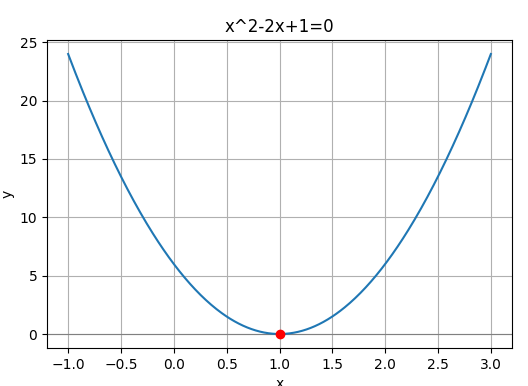
\includegraphics[height=0.4\textheight, keepaspectratio]{figs/parabola.png}
\captionof{figure}{Graph}
\end{figure}
\end{document}